
\chapter{Background and Related Work}

This chapter will establish the foundation of Persuasive recommendation system along with active learning and critiquing approach. Prior to in depth analysis, it will provide important background information along with some required definitions. Additionally, related work will presented, as the chapter proceed further to the end.

\section{Definitions}

\subsection{Recommender System}

Recommender Systems (RS) are search tools, which supports user decision-making by providing the suggestion that, are according to their interests. Such systems are in widely use from social networking to e-commerce sites in order to achieve different purposes. In e-commerce site, they help not only to serve the customer by suggesting items according to their preferences but also support business to improve in its sale. On the other hand in social network site, to suggest friends or pages like according to user preferences. According to Ricci \cite{ricci2010mobile} "RS are information search tools that have been recently proposed to cope with the "information overload" problem, i.e., the typical state of a web user, of having too much information to make a decision". Proposed solution \cite{resnick1997recommender} is an intelligent system that suggests the product or service that fulfill the user’s preference in given context or situation. Suggestions provided by such systems are depended on the model how they are keeping information. Majority of RS are typically community based. In this kind of modeling suggestions are depend about item popularity among the user. Where popularity is calculated by ratings. Important question that arise in such systems are to find item accuracy according user preferences. On the other hand Personalized models are used that depends on the various factors which includes user’s preferences, history of bought/liked items, or the items the user has ranked in the past. Various techniques are use in the developing of recommender system. Classification of recommendation systems \cite{ricci2011introduction} will be discussed as follows.

\subsubsection{Content-based filtering}

In this technique recommendations are based on user preferences. System recommend items that similar to once's liked by user. Item similarity is calculated by features associated with the compared items \cite{ricci2011introduction}. For example, if a user has rated positively, recipe A under the category of sweets then next suggestion that is provided by the system is one which is similar to one user has liked before.

\subsubsection{Collaborative-based}

Collaborative filtering is a technique in which system find the correlation between item and user, based on other user’s feedback having a similar taste in past \cite{ricci2011introduction}. Initially system calculates all similar taste users for the current user and calculate the recommended item that contains either rated or liked by other users having similar taste. Importantly in this approach item speciation will not be considered. For instance, if user like recipe A then next recommendation would be recipe that there are other users who liked recipe A also liked recipe B.

\subsubsection{Demographic}

Recommendations are generated according to user demographic profile. Recommendations can be produced for different demographic niches by combining the ratings of users in demographic clusters \cite{mahmood2007towards}. For example, suggestion provided by the systems are shown according to user’s age. 

\subsubsection{Knowledge-based}

In knowledge-based systems item recommendation is based on domain specific knowledge, which justifies how certain item features meet according to user’s preferences \cite{ricci2011introduction}. Importantly, it uses predication techniques namely Case-based reasoning which reuses the cases past cases that are similar to current case in order to identify item set of recommendation.

\subsubsection{Community-based}

Type of recommendations provided by this kind of system based on preference of user friends. According to Ricci research \cite{ricci2011introduction}, People tend to rely more on recommendations provided by friends rather than on recommendations from anonymous individual having similar taste. Such type of RS model relies on user’s social relations including preference of user’s friends. Suggestions depend on rating that is provided by user’s friends.

\subsubsection{Hybrid Recommender Systems}

Hybrid system is a fusion of any two or more techniques motioned above. Ricci \cite{ricci2011introduction} explains the motivation behind such system to avoid the limitation of one technique. For instance, Collaborative filtering have cold startup problem i.e. they are unable to suggest those items, which have no ratings. On the other hand Content-based doesn’t have such limitation by combination of both approach new hybrid system can be formed. Similarly, Burke and Robin \cite{burke2007hybrid} proposed the combination techniques to create a new hybrid system.

\subsection{Contexts}
Recommendation techniques used by traditional system relies on vector of item rating and user preferences. According to Suchman \cite{suchman1986plans} these approaches ignores the notion of “situated actions” which infers that user have particular context and item preference within one context may be different from another context\cite{adomavicius2011context}.
Absence of context may lose information predictive power because of aggregation of multiple contexts. For instance user wants to buy cloths for his child. Instead of given him child dress system suggests dresses according to user choice because of incomplete contextual information.\newline

Since context is a multi dimension topic therefore vast amount of research has been done in area, narrowing down role of context in recommender system, context can be defined as all information according to given situation. One of the early definitions of context in terms of operation \cite{schilit1994disseminating} defined as where you are, who you are with, and what resources are nearby.  As research further increases, new and most sited definition of context according to Adomavicius \cite{adomavicius2011context} “Any information  that  can  be  used  to characterize  the  situation  of  an entity.  An entity is a person, place, or object that is considered relevant to the interaction between a user and an application, including the user and applications  themselves”. Also, Dourish, P. et al., \cite{dourish2004we} while observing the uses of context they classified into two views namely \textit{representation} and \textit{ interaction } views. They assumed four key assumptions for describing representational view. Context is independent from underlying activity, delineable, stable and in a form of information. According to this view, context can be known prior as it is a set of observable attributes and structure of these attributes does not change with respect to  time. Futhermore, \cite{dourish2004we} while observing the uses of context they classify into two views namely \textit{ representation } and \textit{ interaction } views. They assume four key assumptions for describing representational view context is independent from underlying activity, delineable, stable and in a form of information. According to this view, context can be known prior, as it is a set of observable attributes and structure of these attributes does not change with respect to time. On the other hand interactional view features are dynamic. It assumes that context and activity have a relationship.\newline

Adomavicius \cite{adomavicius2011context} ascertain \cite{dourish2004we} claims on categories  and  explains recommender system can have different types of knowledge, which may include the exact list of all the relevant factors, their structure, and their values, about the contextual factors. He classifies the knowledge of a recommender system about the contextual factors into three categories; \newline

\textit{Fully observable}; refers to explicit knowledge of structure and values of contextual factors of application at the time when recommendations are made. These factors refer as Purchasing Purpose, Shopping Companion and time. For example, User wants to buy shirt, besides having information of selling point and item. Theses may include information about the time, for whom. \textit{Partially observable}; application has some of information about the context explicitly. For instances, Purchasing Purpose, Shopping Companion and time, all information given but the structure is missing. \textit{Unobservable}; no information regarding contextual information is provided explicitly. Utilizing only the latent knowledge of context in an implicit manner makes recommendations. For example, the recommender system may build a latent predictive model, such as hierarchical, linear or hidden Markov models, to estimate unknown ratings, where unobservable context is modeled using latent variables.\newline

Furthermore, Adomavicius \cite{adomavicius2011context} find out the dependency of contextual factors over time and classify them into categories. \textit{Static}; The relevant contextual factors and their structure remains the same (stable) over time. \textit{Dynamic}; contextual factors change in some way.

\begin{figure}[h]
	\centering
	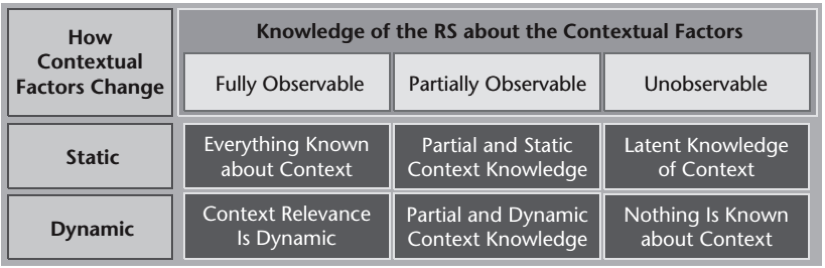
\includegraphics[width=.98\linewidth]{figures/ch2_context_dimensions.png}
	\caption{Contextual Information Dimensions.} 
	\cite{adomavicius2011context}
	\label{fig:ch2_context_dimensions}
\end{figure}

\subsubsection{Representing and Modeling Context}

Classical recommendation system has the prediction problem in which user’s rating for item reflects the degree of user preferences. Therefore, a recommender system tries to estimate a rating function.

\begin{equation} 
R : Users x Items \rightarrow Ratings
\end{equation}

It’s a 2D matrix of user-item to an ordered set of rating values. Where "R" a general-purpose \textit{utility} (or preference). Since the value of "R" is partial function therefore rating of all user-item are not known which arise the predication problem.

\begin{equation} 
R : Users x Items x Contexts \rightarrow Ratings
\end{equation}

In contrast, context aware recommender have additional evidence to estimate user preference on unseen item. Contextual evidence can be applies to input function and viewed as “multidimensional”. Where, any inforsmation related to data and user can be refer as Contextual information

\subsubsection{Paradigms for Using Contextual Information}

According on algorithm approaches of context aware recommendation, represents in form of \textit{U x I x C x R}, Where U is for User, R denotes rating, C is contextual dimension, and produce contextual recommendations list i1, i2, i3 ... for each user u. Figure \ref{fig:ch2_context_recommender_system_paradigms} illustrates the Paradigms used in processing Contextual Information. These are categories as follows:\newline

\textit{Contextual prefiltering} In this filtering Context is applied an input. With the help of any classical 2D recommendation data selection approach, applies current context which is used for selection of relevant ratings and dataset.\newline

\textit{Contextual postfiltering} Prediction of rating is applied with the help of traditional 2D recommender system technique. On the resultant set of recommendation applies the context for each user. \newline

\textit{Contextual modeling} directly integrates the contextual information in the modeling technique as part of the rating estimation. .\newline


\begin{figure}[h]
	\centering
	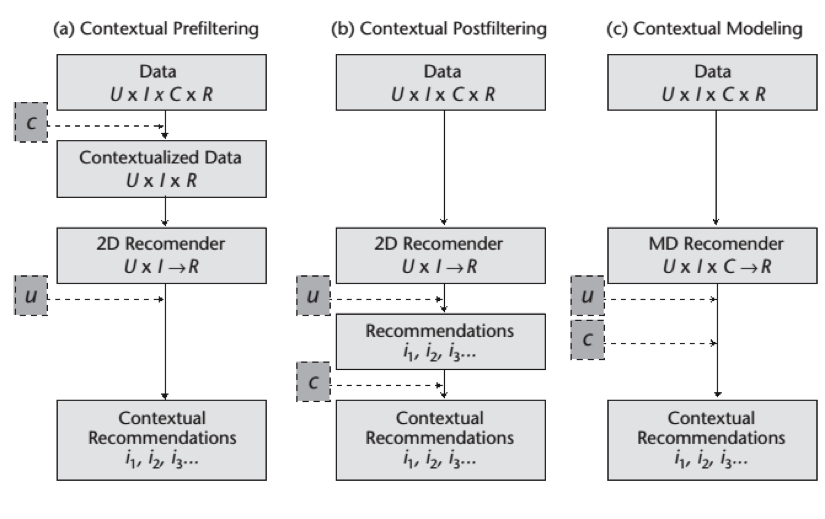
\includegraphics[width=1\linewidth]{figures/ch2_context_recommender_system_paradigms.png}
	\caption{Paradigms for Incorporating Context in Recommender Systems.}
	\cite{adomavicius2011context}
	\label{fig:ch2_context_recommender_system_paradigms}
\end{figure}


\subsection{User Profiling}

User profiling is process of acquiring information about the user, which helps in constructing the user model. Rate of acceptance and effectiveness of recommendation will effect how much system has information about the user. Tang \cite{tang2010combination} explains as  In the context of software applications, a user profile or user model comprehends essential information about the user. It also refers and digital representation of person in a system and hold the person’s preferences. Variations in user profile content depend on application. Some applications depend on demographic information of user while other relies on rating, liking, disliking or other preferences. Also, consideration of user interaction and behavior take plays an important role for providing precise recommendations.\newline

Schiaffino \cite{schiaffino2009intelligent} stated that discovery of differences and similarities in interests among users is a key to provide personalized recommendations  Which implies that application users have different preferences and interests to achieve their goals which leads to importance of creation of user profile in order to find out relationship between user according to their interests. Content of user profile depends on application domain and variations are presents application. Categorically there are two methods to gather content of user profile. First method is manually, in this technique users are being interviewed, fill the some form or questionnaires. For instance asking about his demographic profile like where he is form, which dishes he likes or rating based questions like how frequently he eats junk food? On the other hand by mean of implicit learning about user preference which requires artificial intelligence (AI) techniques like Case-based reasoning, Bayesian Networks, Artificial neural networks. Most of these techniques are beyond the scope of this work so they will not be described in more details. Fundamentally there are two different alternatives to build a user profile; either the information is obtained explicitly from user or implicitly through the observation of user’s actions. The next section describes these alternatives.\newline

\subsubsection{Explicit Profiling}

Explicit profiling often known as explicit user feedback is the simplest way of gathering information about users. In this technique, user has to fill questioners in order to develop profiles. Profiles developed by this techniques are totally depends on the questioner. Normally, data contains demographic information regarding the user like name, age, location and other preferences. Gauch \cite{schiaffino2009intelligent} suggests input methods that allows user to rate item according to their interest. Alternatively system can provide check box and text field in order to get preference of user. \textit{HTML forms, Questionnaires, Rating, User preference and Touch sensors} are some techniques  user to obtain explicit profile. Where as, the limitation of this technique is that it requires user time and willingness to provide their data.  Some user has reservation in regards to provide their personal information because of potential privacy concern. However user’s preference can always be determine via this technique.\newline

\subsubsection{Implict Profiling}

Implicit profiling is also known, as implicit user feedback is another approach for building user profile. It is popular and widely used methodology to develop user profile based on user ‘s acquired information. Mostly profiles are derived form monitoring or observing user activities.  Information acquires by the system helps them to ensure the given recommendation is according to user interest. For example popular website for watching video YouTube. It recommendation is made on similar to those video is watch by user in past.  Single-sign-on (SSO) \cite{hursti1997single} one the most common methodology for user registration. Since the information is implicit they may contains user demographic information. Similarly user preference like, dislike, location can be fetch by integrated related third party services. Information obtain form this mechanism plays an important role in personalized recommendation system. \ textit{Search logs, Browser cache and User monitoring agents} are some techniques used to generate implicit profile. Main advantage of this technique user doesn’t have to enter form and provide their information. Kelly \cite{schiaffino2009intelligent} provides an overview of standard techniques that are help to build user profile and information types about the user that can be in inferred from user’s behavior.\newline

\subsection{Conversation-based Critiquing Recommenders}

Recommender systems may also vary in the function to the extent that user can get engage in the dialogues. In traditional techniques data was collect once and terminate after recommendation are made. Assumption of these approaches is user know all his preferences at the beginning which was not the case. Whereas, user taste may change over time and he want to interact with different option. Smyth \cite{ mcginty2003role} handles this problem and called “Conversational recommendation system” (CRS). He states that CRS have their origins in conversational case-based reasoning (CCBR) which apply similar techniques to elicit query information in problem solving domains and diagnostic tasks.” It is an interactive approach in which user preferences are establish through conversation session. At first initial set of recommendations are given to the user. System adapts the user feedback to further enhance the recommendations. Smyth \cite{ mcginty2003role} distributed feedback into three categories.\textit{ Rating-based} in this approach user provides rating for an specific item.\textit{ Critique-based} where user add constrain over item features.\textit{ Preference-based } in which user indicates its preference for one particular item over the others.\newline

\subsection{Active Learning}

Active learning (AL) is a methodology to learn about user’s preference by asking him/her to rate a number of item knows as training point \cite{ rubens2011active}. Data is formed by model that approximates user’s preference. It is useful where user’s preferences are change with respect to context.  Rashid \cite{rashid2008learning} explains that objective of AL may varies according to objectives of recommendation systems.  For example, what is important in the recommender system being built? The difficulty of signing-up (user effort)? If the user is happy with the service (user satisfaction)? How well the system can predict a user’s preferences (accuracy)? Furthermore, this approach can solve cold startup problem in an effective manner. Figure \ref{fig:ch2_active_learning} explains how interactive process works in order to obtain training data, unlike passive learning, where data is simply given to system in a linear fashion. Rubens \cite{ rubens2011active} categorized AL method according to their primary goal.  

\begin{figure}[h]
	\centering
	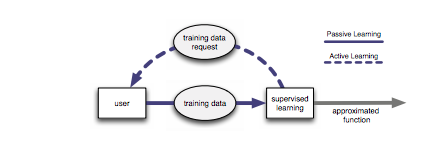
\includegraphics[width=1\linewidth]{figures/ch2_active_learning.png}
	\caption{Active vs Passive Learning}
	\cite{ rubens2011active}
	\label{fig:ch2_active_learning}
\end{figure}

\subsubsection{Instance-based Methods}

In kind of approach points selection is relies on their properties in an attempt to predict user’s rating by the closet match to other user, without have explicit knowledge about underlying model \cite{adomavicius2005toward}. Whereas, it assumes that under consider model any data and rating predictions are accessible.

\subsubsection{Model-based Methods}

In this methodology point selection is based on best construct model that explains data supplied by the user to predict user ratings \cite{adomavicius2005toward}. Similarly, select point are used to maximize the reduction of expected error of the model. Whereas, it assumes that in addition to any data available to instance-based methods, the model and its parameters are also available. 

\subsubsection{Modes of Active Learning: Batch and Sequential}

Since the expectation of user is to high for the system while they are performing interaction. They expect immediate output from the system. One common approach is to recalculate the rating of item once user rated single item, known as sequential mode. However another possibility is that to allow user to rate several features of items or rate several item before model readjustment known as batch mode. As immediate reflection of data in sequential mode is an advantage but cost of interaction will always effect. Therefore, trade-off exists between Batch and Sequential AL: the usefulness of the data vs. the number of interactions with the user. 

\subsection{Persuasive Recommedations}

Traditionally, prevalent research in recommender systems has been focused on algorithms development and evaluation that provide precise recommendations\cite{xiao2007commerce}.The presumption behind the algorithm that its accuracy contribute to the quality and acceptance of the recommender systems has been changed lately\cite{nanou2010effects}. Context and profiling techniques are also emerged as an important pillars.Additional factors which are important and should be focus on is presentation of recommendation so that user can interact with the system in more continent fashion\cite{nanou2010effects}, transparency of system or explain working of system to the end user\cite{sinha2002role}, persuasion\cite{pu2012evaluating} and recommendation’s novelty\cite{cremonesi2012investigating}. Fogg \cite{fogg1998persuasive} defines persuasion as \textit{the attempt of changing people’s attitudes or behaviors or both}.However, explanation of recommendation also have influence on user \cite{mcsherry2005explanation} \cite {herlocker2000explaining}.

\subsubsection{Persuasion factors}

Aristotle in Rhetoric \cite{gkika2014persuasive} was the first one how talked about persuasion. Furthermore, he claims \ textit { ethos/character of the speaker},  \textit { message’s receiver pathos/emotions} and \ textit{ logos/argument} are the main elements that plays an important role in persuasion. Since, difference of opinion exists in factor of recommendation. The mot cited one is  Cialdini’s \cite{cialdini2009influence} known as 6 Influence Principles (also known as Six Weapons of Influence) and if they implemented in a system then effect of persuasion increase. Theses principle include; \ textit{ Reciprocity} (humans have the tendency to return favours), \ textit{ Commitment }(or consistency: people’s tendency to be consistent with their first opinion), \ textit{ Social proof }(people tend to do what others do), \ textit{ Scarcity} (people are inclined to consider more valuable whatever is scarce), \ textit{ Liking }(people are influenced more by persons they like) and  \ textit{ Authority} (people have a sense of duty or obligation to people who are in positions of authority). Where Figure\ref{fig:ch2_communication_persuasion_paradigm} indicates effect of Communication Persuasion Paradigm\cite{yoo2012persuasive}.

\begin{figure}[h]
	\centering
	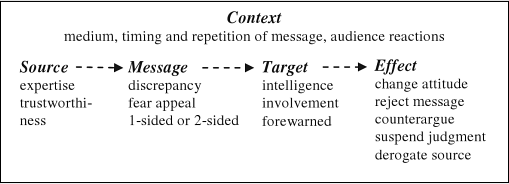
\includegraphics[width=1\linewidth]{figures/ch2_communication_persuasion_paradigm.png}
	\caption{Communication Persuasion Paradigm}
	\cite{yoo2012persuasive}
	\label{fig:ch2_communication_persuasion_paradigm}
\end{figure}

\newpage
\subsubsection{Explanations in Recommender Systems}

An explanation consider an additional information provided by system output to achieve certain goals \cite{tintarev2011designing}. Explanation persuade user to try or buy recommended item\cite{tintarev2012evaluating}. Several aspects should be considered in order to introduce explanation into the system. Following are the seven goals for explanation in recommendation system\cite{tintarev2007survey}.

\begin{enumerate}
	\item \textbf{Transparency} in recommendation system helps to understand how the recommendations are generated and how overall system mechanics\cite{tintarev2007survey}. Furthermore, it allow user to check the quality of system and in case anomalies user have an idea why system is given this result. Let consider an example, suppose system recommends a movie in comedy genre for a particular actor although user is not interest in it. System will provide an explanation you like some movies of this actor that’s why it is in your recommendation.
	
	\item \textbf{Scrutability} allow user to misguided assumptions made by system. Since user preferences may always change due to contextual factors. Therefore, it is important that explanations enable the user to understand what is going on in the system and let them exert control over the type of recommendations. Scrutability is related to the established usability principle of User Control\cite{nielsen1990heuristic}.
	
	\item \textbf{Trust} increase users’ confidence in the system\cite{tintarev2007survey}. Trust could also relies on recommendation algorithm\cite{ mcnee2003interfaces}. Studies suggested that trust is related to transparency and increase the possibility of interaction with the system.\cite{ elfernig2006empirical}. If users find system trustworthy then they are intent to return back to the system\cite{felfernig2006empirical}. 
	
	\item \textbf{Persuasiveness} convince users to try or buy \cite{tintarev2007survey}, where as it may increase user evolution of the system. It allow user to gain benefits form the system rather than relied on other individuals.

	\item \textbf{Effectiveness} helps user to make good decision \cite{tintarev2007survey}. Effectiveness is totally depends on recommendation algorithm. It also helps user to evaluate the quality of recommendation according to their preferences and also discard those item, which are not related to taste.  
	
	\item \textbf{Efficiency} help users make decisions faster \cite{tintarev2007survey}. Nielsen describe efficiency is an establish usability principle and explain it is ability of system to help user in fast decision making while selection of best suited item\cite{nielsen1990heuristic}.
	
	\item \textbf{Satisfaction} is the ability to make system fun while user is interacting with the system \cite{tintarev2007survey}. Similarly, providing poor recommendation tends to decrease a user’s interest \cite{ tanaka2000multi} or acceptance of a system\cite{herlocker2000explaining}.
	
\end{enumerate}

\subsection{Mobile Recommender Systems}

With the technical advancement and features like computers, mobile phones have become a primary platform. By Combining with recommendation system it become a key tool for business and users. Due to this trend personalization in recommendation become more focus. Hence, it is important to understand the capabilities of mobile and how the information will access and displayed on mobile phone for usability prospective\cite{nielsen1990heuristic}. Schiller \cite{schiller2003mobile} describe the mobile recommendation system in three dimensions. According to him each one has its own impact on system usage and functionality. Furthermorem these dimensions are independent but there are examples for all the possible combinations of these dimensions. These are stated as follows:

\begin{enumerate}

	\item \textbf{Device portability} describes as information can be access from any location without bounding it to any specific location. Furthermore, user experience will be the same regardless of the location it is being accessed from. 
	
	\item \textbf{User mobility} refers to information is access for mobile device, like smartphone and tablets. On the other hand there is some constrains regarding the screen sizes and how information will be displayed such devices.
	
	\item \textbf{Wireless connectivity} refers to all the information, which is access by the mobile, is via wireless technology such as wifi, 3G and LTE.
	
\end{enumerate}

\subsubsection{General Issues}

Beside all the advancements and opportunities provided by mobile devices there are some limitation that exists and state as follows:

\begin{enumerate}
	
	\item \textbf{Resource limitation}\newline 
	Mobile devices offer less memory and power consumption as computer to standard computing machine for example desktop computers.\cite{ricci2010mobile}. 
	
	\item \textbf{Connectivity}\newline 
	Since the communication in mobile system is depends on wireless connectivity therefore, high amount interruption and noise occur. Furthermore,  data rate is also very low as compare to standard wire communication.\cite{ricci2010mobile}.
	
	\item \textbf{Battery life}\newline
	It is the most biggest and concern challenge among all. Although significant research and improvement has been performed in battery life of mobile device but a lot needs to be done for providing better battery life.\cite{ricci2010mobile}.
	
	\item \textbf{Fragmentation}\newline 
		Fragmentation refers to different screen sizes of devices. Since there are more than thousands of devices that exist having different screen size and resolutions. It is a challenge for developer to support all of them.\cite{ricci2010mobile}.
\end{enumerate}

\section{Related Work}
This section gives an overview of previous work and related papers on the respective domain.

\subsection{User's Food Preference Extraction for Personalised Cooking Recipe Recommendation}

Mayumi, Mari and Shinsuke \cite{ueda2011user} design system to enlighten importance of personalized recipe recommendation system which is based on user’s food preferences. In this research user’s preferences are gathered by his browsing and cooking history. Recommendations provided by this system is not depends on what user ate in past. Moreover, system does not require particular action of user to collect his preferences.  Figure \ref{fig:ch2_ueda2011user} illustrate the idea estimating user’s favorite ingredients. Their approach breakdowns the recipes into like and dislike ingredients set. It calculate ingredient the score by incorporating the frequency of that ingredient in the dishes that has eaten by user and consider them in like ingredient. Whereas, ingredient is consider as dislike by user if he never browsed the recipe details or never cooked. Since system is working on implicit profiling therefore unable to consider addition context and preference of user while generating recommendations.

\begin{figure}[h]
	\centering
	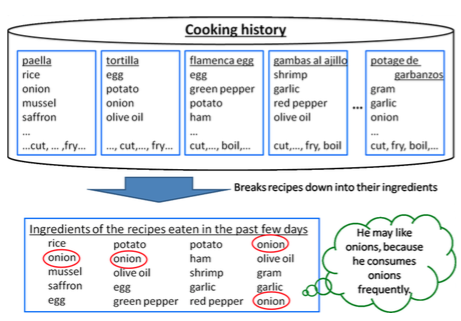
\includegraphics[width=1\linewidth]{figures/ch2_ueda2011user.png}
	\caption{Extracting the favorite ingredients using cooking history}
	\cite{ueda2011user}
	\label{fig:ch2_ueda2011user}
\end{figure}

\subsection{Knowledge Base Framework for Development of Personalised Food Recommendation System}
Suksom, Napat and Buranarach \cite{suksom2010knowledge} focus on personalized food recommendation system aims to provide dietary recommendation based on individual diet and preferences by using knowledge base recommendation technique. Where as, knowledge based depends on ontology and rule-based knowledge development. Figure \ref{fig:ch2_suksom2010knowledge} gives an overview of system. All user preferences are set initially and recommendations are based on his heath preference infers system not supports critiquing approach.  

\begin{figure}[h]
	\centering
	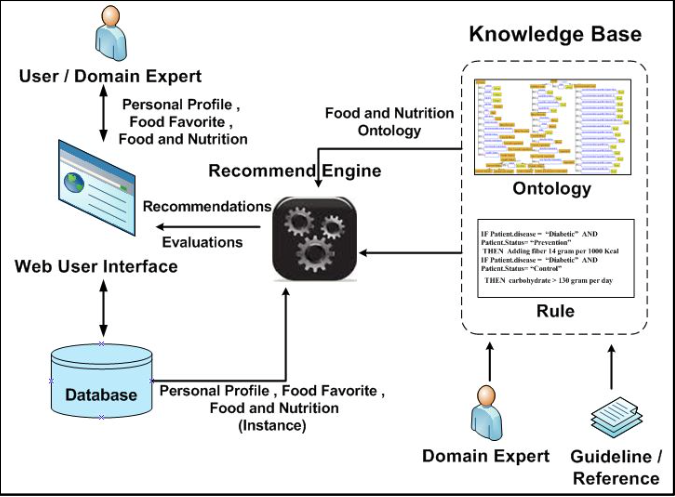
\includegraphics[width=.70\linewidth]{figures/ch2_suksom2010knowledge.png}
	\caption{Knowledge-based framework for the food recommender system}
	\cite{suksom2010knowledge}
	\label{fig:ch2_suksom2010knowledge}
\end{figure}

\subsection{Recommending Food: Reasoning on Recipes and Ingredients}

Focus of the research is to investigate recipe recommendation system techniques by applying different recommendation techniques \cite{freyne2010recommending}. Initially with collaborative filter approach with simple break down to relate recipe and ingredients result were not so good but by applying content based approach there were significant improvements in result. For optimal solution they used hybrid approach of content-based and collaborative filter. Summary of their work is stated as after breaking down the recipes into ingredients, give and compute score ingredient score, applying collaborative filter to narrow down the ingredient score and finally applying content based approach in which prediction of recipe rating is examine by the score of individual ingredients. This approach conveys the basic idea recipe recommendation system. With the addition of user preference and their feedback it could achieve more.

\subsection{Recipe recommendation using ingredient networks}

Teng, Chun-Yuen and Lin, Yu-Ru and Adamic, Lada \cite{teng2012recipe} research permits collaborative recipe generation and modification. Recipes data are gathered according to regional preferences and modification is done by individual ingredient preferences. By this approach two kinds of networks are created one is ingredient complement and other is ingredients substitution. The network suggests which substitution of ingredient increases the taste of the recipe and gives those recipes, which is high rated by user. System uses collaborative filter approach along with data mining techniques. System does not have diet specific recipes according to user preference nor consider any user context. 

\subsection{Critique-Based Mobile Recommender Systems}

Ricci \cite{ricci2005critique} illustrates the critique based  mobile base recommendation in the domain of travel. Motivation behind this research to collect collects user preferences via critique with low amount of user effort. According to this research it is an advantage to collect user preference via critiquing and it is relatively fast. Figure \ref{fig:ch2_ ch2_ricci2005critique} shows how the critiquing is perform. On the other hand it does not support reactiveness if  use preferences has changed. It gives the basic idea how to gather information regarding user preferences in our system. 
 
\begin{figure}[h]
	\centering
	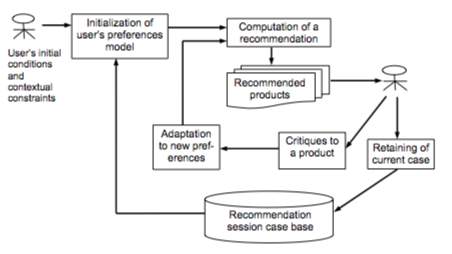
\includegraphics[width=.70\linewidth]{figures/ch2_ricci2005critique.png}
	\caption{Critique-Based recommendation model}
	\cite{ricci2005critique}
	\label{fig:ch2_ricci2005critique}
\end{figure}


\subsection{Active Learning Strategies for Exploratory Mobile Recommender Systems Interactive Explanations in Mobile Shopping Recommender Systems}

Motivation behind this approach to developed a explorative shopping mobile recommendation system by using conversation-based active learning approach \cite{lamche2014active}. It uses the utility-based context and critiquing for feedback. Recommendations improvements are done by two-step critiquing process which illustrating in at Figure \ref{fig:ch2_lamche2014active_1}. Critiquing process is relies on either positive or negative feedback. Figure \ref{fig:ch2_lamche2014active_2} show the refine model of recommendation in a system. On the other hand it does not deals with the context and tell user why this recommendation is given to him. 

\begin{figure}[h]
	\begin{subfigure}{.49\textwidth}
	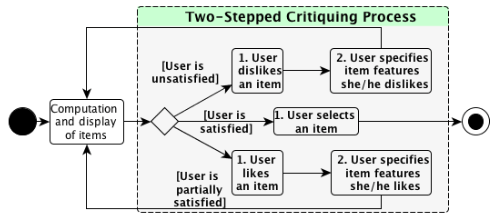
\includegraphics[width=.9\linewidth]{figures/ch2_lamche2014active_1.png}
	\caption{The two-stepped critiquing process}
	\cite{lamche2014active}
	\label{fig:ch2_lamche2014active_1}
	\end{subfigure}
	\begin{subfigure}{.49\textwidth}
	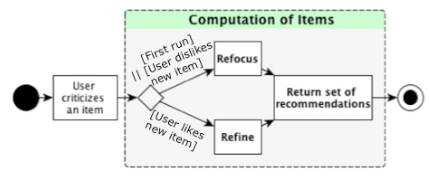
\includegraphics[width=.9\linewidth]{figures/ch2_lamche2014active_2.png}
	\caption{Active Learning recommenation model}
	\cite{lamche2014active}
	\label{fig:ch2_lamche2014active_2}
	\end{subfigure}
	\caption{Active Learning Strategies}
	\label{fig:lamche2014active}
\end{figure}

\subsection{The Persuasive role of Explanations in Recommender Systems}

Ricci, Francesco and Nguyen\cite{gkika2014persuasive} design and analyze a movie recommendation system in which they tried to recommend those movies that are according user’s interest. It helps them to understand the persuasion effect that users are willing to accept recommendation or not. System is design to suggest persuasion recommendation based on Kaptein’s \cite{kaptein2012adaptive} methodology and follows the approach of six(6) best-matching explanation \ref{table:best-matching-explanation} to provide Persuasion Principle. This approach is does not support active learning and critiquing approach not handling of current context.

\begin{table}[ht]
	\centering % used for centering table
	\begin{tabular}{p{2cm} p{12cm}}  % centered columns (4 columns)
		\hline\hline %inserts double horizontal lines
		Influence Strategy & Explanations \\ % inserts table
		%heading
		\hline % inserts single horizontal line
		Reciprocity & A Facebook friend, who saw the movie that you suggested him/her in past, recommends you this movie \\ % inserting body of the table
		Scarcity & The recommended movie will be available to view from 15/1/2014 to 31/1/2014 on cinemas \\
		Authority & The recommended movie won 3 Oscars\\
		Social Proof & 76"\%" users rated this movie with 4 to 5 stars\\
		Liking & Your Facebook friends like this movie \\
		Commitment & Watch this movie and you may change your mind about this kind of movies\\ [1ex] % [1ex] adds vertical space
		\hline %inserts single line
	\end{tabular}
	\caption{Best-matching Explanations on each Influence Strategy}
	\label{table:best-matching-explanations}
\end{table}



